\chapter[Revisão Bibliográfica]{Revisão Bibliográfica}
% ----------------------------------------------------------
%Ataques distribuídos de negação de serviço (do inglês, DDoS) figuram uma das principais ameaças de segurança atualmente. Organizações perdem financeiramente e principalmente tendem a ter seu valor questionado quando são vítimas de invasores na rede.
\section{Segurança da Informação}
Uma ameaça trata-se de um potencial para violação de segurança quando há uma circunstância que pode quebrá-la, causando danos a um serviço/\textit{host}. Exemplos de ameaças são: \textit{malwares}, ataques de negação de serviço, envio de pacotes com falso endereço origem. Uma ameaça explora uma vulnerabilidade no alvo para obter s informações que deseja ou mesmo tornar o serviço indisponível, ou seja, ocorrendo a violação da segurança no alvo que é o ataque. Um ataque pode ocasionar, por exemplo, a destruição dos dados, perda da integridade, quebra de equipamentos, dentre outros incidentes. Um incidente, por sua vez pode causar prejuízo financeiro para a imagem do alvo, além de causar indisponibilidade do serviço. A \figref{fig:ameacas} mostra uma síntese desses conceitos.   

 \begin{figure}[ht]
 	\centering
 	\caption{Fluxo explicativo de uma ameaça }
 	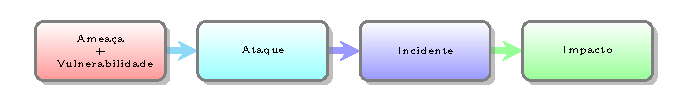
\includegraphics[width=0.8\textwidth]{figs/ameacas.pdf}\\
 	{Fonte: Elaborada pelo autor.}
 	\label{fig:ameacas}
 \end{figure}
 
 \section{Ataques DoS e DDoS}

Um ataque de negação de serviço(DoS - Denial-of-Service) torna um componente de rede inutilizável por usuários que estejam consumindo o serviço fornecido. A maioria dos ataques DoS na internet pode ser dividida em três categorias: \cite{kurose}
\begin{itemize}
	\item Ataque de vulnerabilidade: Mensagens são enviadas a uma aplicação vulnerável ou a um servidor, sendo executado em um hospedeiro alvo.
	\item Inundação na largura de banda: O atacante envia um grande número de pacotes maliciosos ao hospedeiro alvo até que o enlace de acesso do alvo se entope, impedindo os pacotes legítimos de alcançarem o servidor. 
	\item Inundação na conexão: O atacante estabelece um grande número de conexões TCP semiabertas ou abertas no hospedeiro alvo. 
\end{itemize}
Já segundo \cite{ddosatacks}, os ataques DoS são classificados em 5 categorias baseadas no protocolo cujo é atacado: Dispositivo, sistema operacional, aplicação, inundação de dados e características do protocolo. O primeiro inclui ataques que podem ser causados ao tirar vantagem de \textit{bugs} ou vulnerabilidades em software. O segundo leva em consideração ataques que aproveitam-se das formas nas quais os sistemas operacionais implementam os protocolos. Ataques baseados na aplicação infectam o alvo por meio de \textit{bugs} específicos da rede e tentam drenar os recursos da vítima. Em ataques baseados em inundação de dados, um atacante tenta usar a largura de banda disponível para mandar quantidades massivas de dados, fazendo com que o alvo processe essa grande quantidade. Por fim, ataques baseados em características do protocolo são caracterizados por tirarem vantagens de certos padrões de protocolo.
 
Um ataque distribuído de negação de serviço (do inglês, DDoS) utiliza as propriedades de um ataque DoS de forma distribuída. Em outras palavras, a indisponibilidade de um serviço é causada por ataques oriundos de um ou mais IPs origem, tornando mais complexo o tratamento e a busca pelo atacante que está propagando a ameaça. De acordo com \cite{WANG2015308}, atualmente os atacantes podem lançar vários ataques DDoS, focando-se nos recursos (largura de banda da memória e CPU) e em aplicativos (aplicações web, serviços de banco de dados). Alguns tipos de ataques DDoS podem ser citados:

\begin{itemize}
	 \item \textit{Smurf}
	 \item UDP \textit{Flood}
	 \item SIDDoS
	 \item HTTP \textit{Flood}
\end{itemize}

\subsection{Smurf}
Ataques DDoS do tipo \textit{Smurf} possuem dois componentes principais que são o uso de requisições ICMP forjadas e a direção dos pacotes para um endereço \textit{broadcast}. O protocolo ICMP é usado para troca de mensagens de controle e pode ser usado para determinar se uma máquina na internet está respondendo. Um exemplo prático desse comando é o ping, onde vc envia mensagens para um IP e recebe uma resposta, sendo do IP alvo, ou por tempo de requisição excedido (\textit{timeout}). Além disso, um IP \textit{broadcast} serve para comunicar-se com todos os \textit{hosts} em um segmento de rede. Assim, os invasores usam pacotes de solicitação de eco ICMP direcionados para endereços de IP \textit{broadcast} para gerar ataques de negação de serviço. Note que esse ataque possui três participantes: o atacante,, um intermediário(que também pode ser uma vitima) e o alvo. Esse intermediário recebe um pacote ICMP direcionado ao IP \textit{broadcst} de sua rede. Se esse intermediário não filtra seu tráfego, muitas máquinas na rede irão receber esse pacote de requisição e responderão ao mesmo por meio de uma resposta eco ICMP, provocando um congestionamento grave na rede \cite{certSmurf}.
\subsection{HTTP \textit{flood}}
Esse tipo de ataque, diferentemente do \textit{Smurf} é realizado na camada de aplicação, pois utiliza o protocolo HTTP. Trata-se de um ataque volumétrico, ou seja, torna um recurso indisponível por meio de uma grande quantidade de informação em uma pequena janela de tempo. Tal ataque pode ser explorado por  usar uma grande quantidade de conexões concorrentes, ou por meio de um grande consumo de banda (como por exemplo vários \textit{hosts} fazendo \textit{download} de um arquivo grande) em uma pequena janela de tempo. Assim, um atacante pode infectar vários \textit{hosts} e comandá-los a realizar um "bombardeio" de conexões em um alvo. Além disso, dentre as várias ferramentas existentes, pode-se citar o LOIC. Tal ferramenta realiza um número de requisições por segundo definido pelo usuário a um alvo. A \figref{sa} mostra seu uso  

\section{IDS}

Para tratar esse tipo de problema, sistemas de detecção de intrusos (do inglês, IDS) são utilizados. Tratam-se de softwares responsáveis  por detectar anomalias na rede, como por exemplo acessos não autorizados e tráfegos mal intencionados. O IDS monitora o tráfego, buscando anomalias e em caso positivo, alerta aos administradores da rede para estes tomarem as medidas corretivas, bloqueando as portas, negando serviço a um IP específico que esteja enviando requisições maliciosas ou fechando serviços que são geralmente utilizados para ataques. Segundo \cite{Ashoor2011}, IDS possuem 3 categorias: 
\begin{itemize}
	\item Sistemas de detecção baseados em assinatura
	\item Sistemas de detecção baseados em anomalias
	\item Sistemas de detecção baseados em especificação
\end{itemize}

O sistema de detecção baseado em assinaturas depende de listas atualizadas com padrões de ataques e assim, será impossível detectar uma ameaça desconhecida ou atualizada. No caso de sistemas baseados em anomalias, depende-se de uma classificação da rede como normal ou anômala, além de conhecer o comportamento normal da rede. Por fim, um sistema de detecção baseados em especificação é responsável por monitorar os processos e caso detecte qualquer comportamento anormal, emitirá um alerta e deve ser mantido e atualizado sempre que houver alguma alteração.

Assim, IDS utilizam alguns conceitos para realizarem seus serviços. Pode-se destacar a definição de objeto de tráfego, o qual significa um conjunto de pacotes em uma determinada janela de tempo. A partir de um objeto de tráfego, pode-se calcular métricas de avaliação da rede. Vale ressaltar que para a obtenção de objetos de tráfego, faz-se necessário o uso de \textit{sniffer}, um analisador de rede que captura o tráfego que entra e sai. Desta forma, os pacotes são capturados e calculam-se os parâmetros do objeto de tráfego.

 


Falar sobre ataques, definir objeto de tráfego, sniffer IDS vulnerabilidades trabalhos relacionaados entropia de shaannon... EXEMPLOS DE AATQUES ddos
   

